\documentclass{article}
\usepackage[utf8]{inputenc}
\usepackage{amsmath}


\title{ CH3 Gaussian Filter \\  Exercise 3 Solution}
\author{zlt1213@gmail.com}
\date{June 2019}

\usepackage{natbib}
\usepackage{graphicx}





\begin{document}

\maketitle

\section{Problem 1}
Let $X_t$ denote the state of the car at time $t$. 
\subsection{Question (a)}
The state vector should be:

$
x_t = 
\begin{pmatrix}
x \\
\dot{x}\\
\end{pmatrix}
$



\subsection{Question (b)}
Goal: State Transition model of $P(x_t | u_t, x_{t-1})$ \\
Solution:\\ \\
Let $u_t$ denote operation at time $t$, then \\
$u_t\sim{N(0, \sigma^2)}$ \\ \\
Suppose during $\Delta t$, the acceleration is constand, thus\\
$\ddot{x_t}=u_t$\\
$\dot{x_t} = \dot{x_{t-1}}+u_{t-1} \Delta t$ \\
$x_t = x_{t-1}+ \dot{x_{t-1}}\Delta t + u_{t-1}{\Delta t}^2/2$\\

$$
X_t = 
\begin{pmatrix}
1 & \Delta t \\
0 & 1 
\end{pmatrix} X_{t-1} + 
\begin{pmatrix}
0.5{\Delta t}^2  \\
\Delta t
\end{pmatrix} \ddot{x}_{t-1}
$$\\
since $u_{t-1}\sim{N(0, \sigma^2)}$, we have $\ddot{x}_{t-1}\sim{N(0, \sigma^2)}$\\

$$A = \begin{pmatrix}
1 & \Delta t\\
0 & 1 
\end{pmatrix}, 
B = 
\begin{pmatrix}
0 \\
0
\end{pmatrix}, 
\epsilon = 
\begin{pmatrix}
0.5{\Delta t}^2 u\\
\Delta t u
\end{pmatrix}
$$ where $u\sim{N(0, \sigma^2)}$\\
as $\Delta t = 1$\\
$$
\epsilon = 
\begin{pmatrix}
0.5u\\
u
\end{pmatrix}
$$
so,
$$
R = 
\begin{pmatrix}
1/4 & 1/2\\
1/2 & 1
\end{pmatrix}
$$\\




\subsection{Question (c)}
Suppose $$ 
\Sigma_0 = 
\begin{pmatrix}
0&0\\0&0
\end{pmatrix}
$$\\ 
For $t = 1, 2, 3, 4, 5$\\
$$ 
\bar{\Sigma}_1 = A\Sigma_0A^{T}+R=\begin{pmatrix}
0.25 & 0.5 \\
0.5  & 1.0
\end{pmatrix}
$$\\
$$ 
\bar{\Sigma}_2 = A\Sigma_1A^{T}+R=\begin{pmatrix}
2.5 & 2.0 \\
2.0  & 2.0
\end{pmatrix}
$$\\
$$ 
\bar{\Sigma}_3 = A\Sigma_2A^{T}+R=\begin{pmatrix}
8.75 & 4.5 \\
4.5  & 3.0
\end{pmatrix}
$$\\
$$ 
\bar{\Sigma}_4 = A\Sigma_3A^{T}+R=\begin{pmatrix}
21.0 & 8.0 \\
8.0  & 4.0
\end{pmatrix}
$$\\
$$ 
\bar{\Sigma}_5 = A\Sigma_4A^{T}+R=\begin{pmatrix}
41.25 & 12.5 \\
12.5  & 5.0
\end{pmatrix}
$$\\



\subsection{Question (d)}


\begin{figure}[hbtp]
\centering
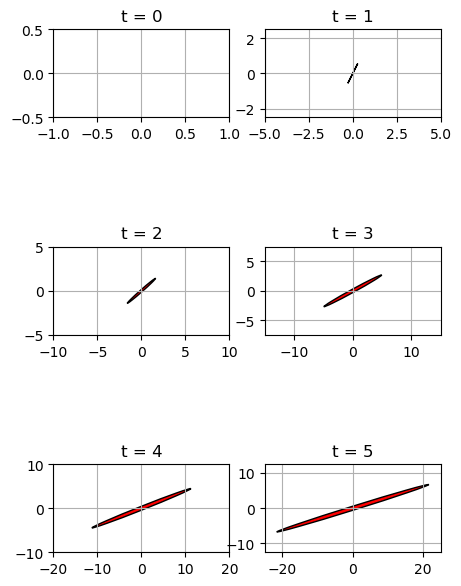
\includegraphics[scale=1.1]{./figures/ch3p1.png}
\caption{Uncertainty Ellipse}
\label{fig:Uncertainty Ellipse}
\end{figure}

\newpage


\subsection{Question (e)}
As $t\rightarrow \infty$, the uncertainty ellipse will keep growing.




\section{Problem 2}
As in Problem 1\\ \\
$
x_t = 
\begin{pmatrix}
x \\
\dot{x}\\
\end{pmatrix}
$

\subsection{Question (a)}

Let $z_t$ denote a measurement, since only the displacement is measured\\
$$
z_t = 
\begin{pmatrix}
1 & 0 \\
\end{pmatrix}
x_t + \delta_t
$$
\\
where $\delta_t \sim{N(0,10)}$ and $Q = [10]$ (a single element matrix).
\\
\subsection{Question (b)}
From problem 1,
$$
\bar{\mu}_5 = \begin{pmatrix}
0 \\ 0
\end{pmatrix},
\bar{\Sigma}_5 =\begin{pmatrix}
41.25 & 12.5 \\
12.5  & 5.0
\end{pmatrix}
$$\\
\\
$$
K_5 = \bar{\Sigma}_5 C_5^{T}(C_5\bar{\Sigma}_5 C_5^{T}+Q_5)^{-1}
$$ where $$
Q_5 = [10], C_5 = [1, 0]^T
$$\\
so\\
$$
K_5 = \begin{pmatrix} 
0.80 \\
0.24
\end{pmatrix}
$$\\
$$
\mu_5=\bar{\mu_5}+K_5(z_5-C_t\bar{\mu_5})\\
=\begin{pmatrix}
4.02\\1.22
\end{pmatrix}
$$\\
$$
\Sigma_5 = (I - K_tC_5)\bar{\Sigma_5}\\
=\begin{pmatrix}
8.05 & 2.44 \\
2.44 & 1.95
\end{pmatrix}
$$
\begin{figure}[hbtp]
\centering
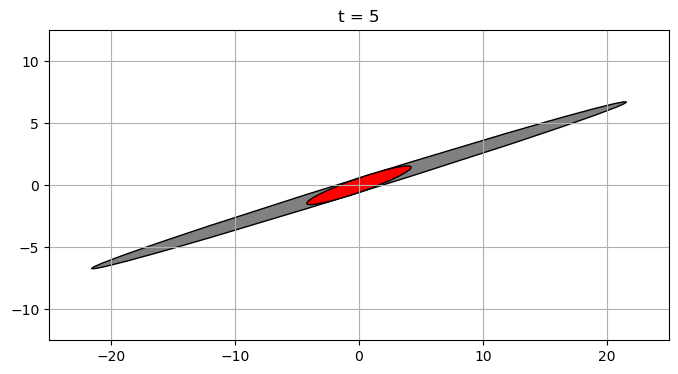
\includegraphics[scale=0.7]{./figures/ch3p2.png}
\caption{Uncertainty Ellipse: Before(Gray) and After(Red) Observation}
\label{fig:Uncertainty Ellipse}
\end{figure}
\\
\\
\section{Problem 3}



















\end{document}